\section{Pre-processing of Matrix}
An Approximate Minimum Degree ordering algorithm (AMD) for pre-ordering a symmetric sparse matrix would result in less fill-in of matrix  Decomposition. The pre-processing stage is done entirely in MATLAB using built-in function amd of MATLAB. Pre-processing of matrix ensures better performance also provides that there will be no divide by zero error in the computation of Decomposition.
AMD Ordering would decrease the floating-point operations, which reduces the compute time. To illustrate the impact following is the matrix before and after AMD ordering on rajat1 Matrix.


\begin{figure}[H]
    \centering
        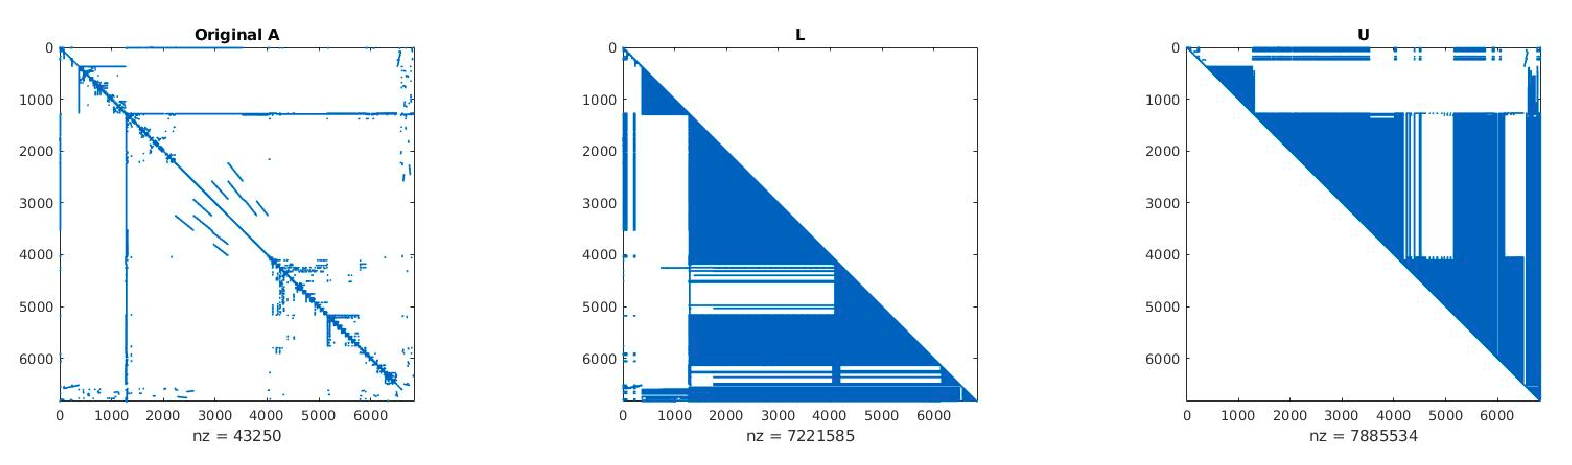
\includegraphics[width = 0.95\linewidth]{./Theory/Original_A.png}
    \caption{Non-zero elements of L and U with original matrix A}
\end{figure}

\begin{figure}[H]
    \centering
        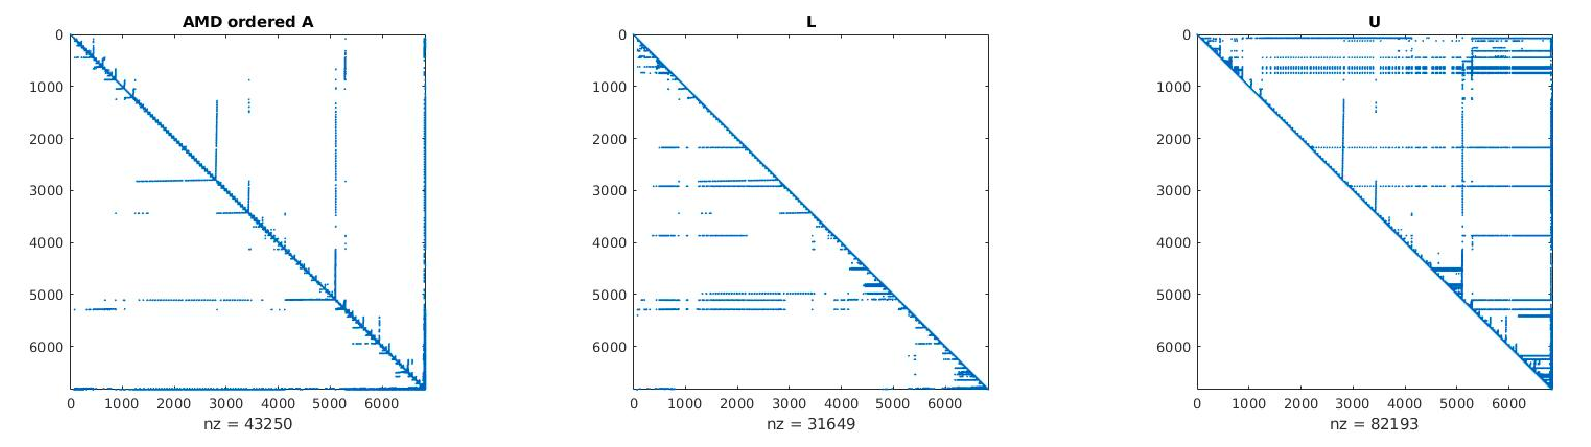
\includegraphics[width = 0.95\linewidth]{./Theory/AMD_A.png}
    \caption{ Non-zero elements of L and U with AMD ordered matrix permuted A}
\end{figure}

The given matrix is a sample matrix given by \cite{SparseSuite}. Circuit simulation matrices from Rajat and Raj.From a company that develops commercial circuit simulation tools.
We can solve a linear problem $Ax = b$ by solving the reordered problem where P is the AMD permutation matrix.
\begin{equation}
    \centering
    (P^TAP)(P^Tx) = P^Tb
    \label{eqn:AMD:ModifiedLinear}
\end{equation}


